\documentclass[a4paper, 10 pt, titlepage]{article}
\usepackage[utf8]{inputenc}
\usepackage[T1]{fontenc}
\usepackage[slovene]{babel}
\usepackage{lmodern}
\usepackage{graphicx}
\usepackage{subcaption}



\title{Nanotorusi}
\author{Tomas Rode \\ Enej Kovač}

\begin{document}
\maketitle

\tableofcontents
\pagebreak

\section{Navodila}

Nanotorus je 3-regularen graf na torusu. Vsak nanotorus lahko dobimo tako, da na šeskotni mreži enačimo nasprotni stranici danega paralelograma. Torej je vsak nanotorus določen z dvema vektorjema v ravnini, $(k,l)$ in $(m, n)$, za katera velja $k^2 + l^2 \neq 0$ in $m^2 + n^2 \neq 0$. Projekt je sestavljen iz štirih podnalog:

\begin{enumerate}
  \item V prvem delu naloge ustvarite funkcijo, ki v \textit{Sage} konstruira nanotorus, za dane $k, l, m$ in $n$.
  \item S pomočjo funkcij v \textit{Sage} preučite nekaj lastnosti nanotorusov: za dan $(k, l, m, n)$ določite število vozlišč, premer, tranzitivnost, ...
  \item Za $v \in V(T)$, poljubno vozlišče nanotorusa, določite število vozlišč na razdaljah $i:\ 1 \leq i \leq \textrm{diam}(T)$. Poizkusite poiskati formulo za dane $i, k, l, m, n$.
  \item Naj bo $T$ nanotorus tipa $(k, l, m, n)$. Ugotovite ali obstaja nanotorus tipa $(k', 0, m', n')$, izomorfen $T$. Če obstaja, ugotovite povezavo med $(k, l, m, n)$ in $(k', m', n')$.
\end{enumerate}

\pagebreak

\section{Funkcija nanotorus}

S pomočjo objektnega programiranja sva v \textit{Sage} zapisala funkcijo, ki konstruira nanotorus s $k, l, m$ in $n$. Na sponjih slikah lahko vidimo nekaj primerov.

\begin{center}
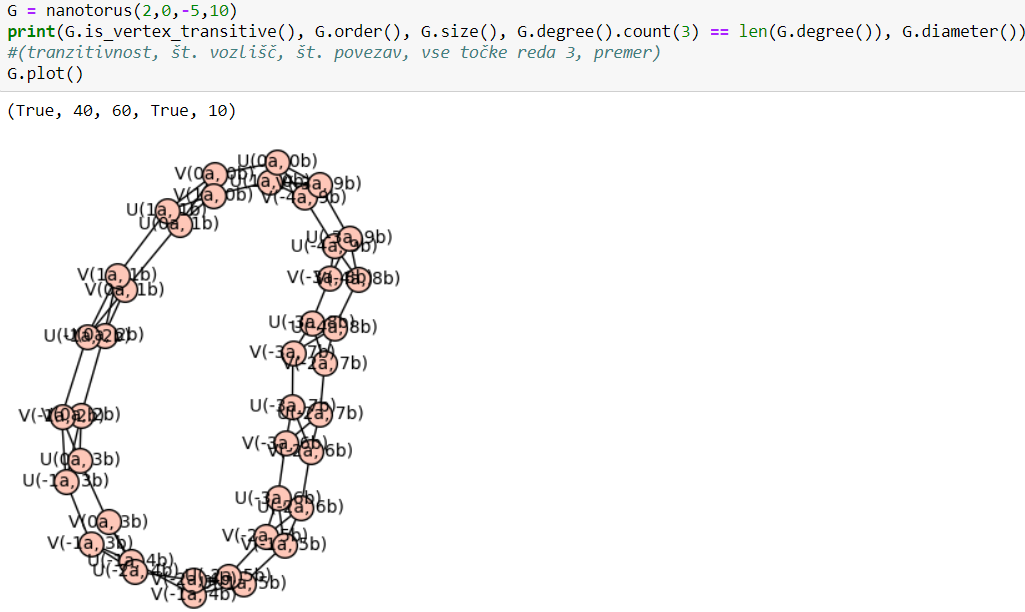
\includegraphics[width=10cm]{nano2}
\end{center}
\vspace{1cm}

Na prvi sliki sva dovolila, da \textit{Sage} prerazporedi točke po prosotru tako, da se čim bolje vidi oblika grafa. Pri tem se nekoliko izgubi šestkotna mreža, na kateri smo graf ustvarili. Pri vsakem grafu sva preverila še tranzitivnost, število vozlišč in povezav, red vozlišč in premer grafa.
\vspace{1cm}

\begin{center}
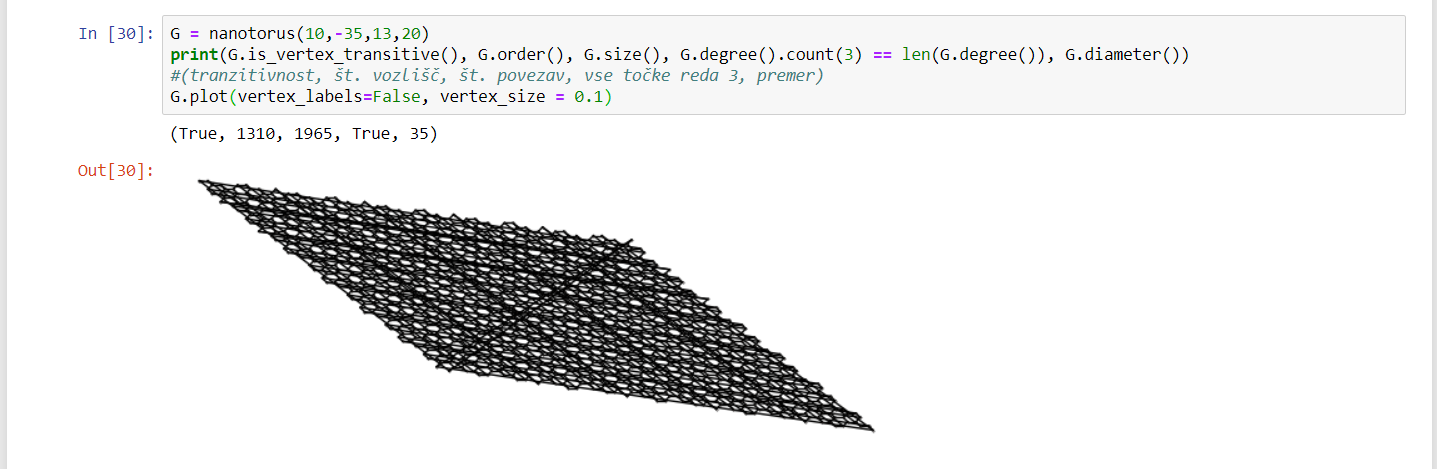
\includegraphics[width=10cm]{nano3}
\end{center}
\vspace{1cm}

Pri drugem grafu sva ohranila koordinate vozlišč na šestkotni mreži. Izmed vseh grafov je torej tukaj izvorna šestkotna mreža najbolj razvidna.
\vspace{1cm}

\begin{center}
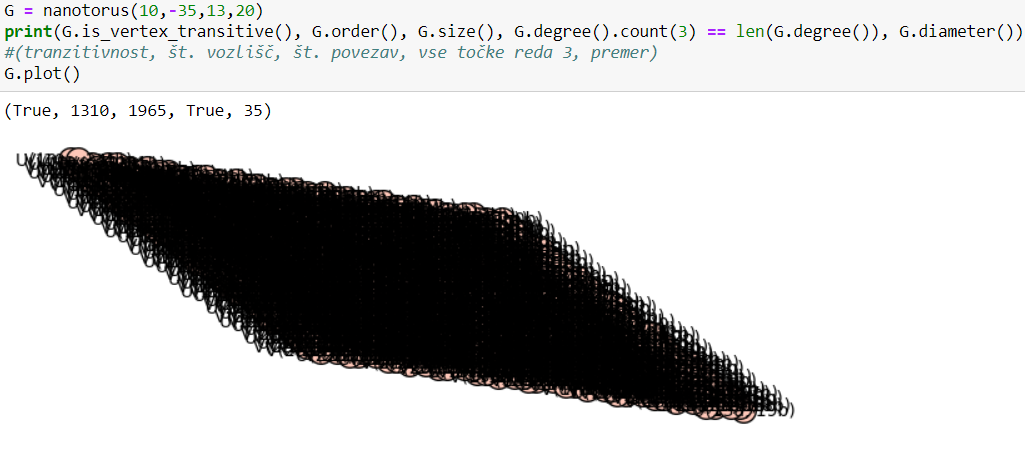
\includegraphics[width=10cm]{nano1}
\end{center}
\vspace{1cm}

Tretji graf ima veliko vozlišč, kar ga dela zelo nepreglednega, omogoči pa, da preverimo omenjene lastnosti nanotorusov tudi za velike grafe.

\subsection{Opis delovanja funkcije nanotorus}

Funkcijo nanotorus sva si zamislila tako, da deluje v naslednjih korakih:

\begin{enumerate}
\item Definicija razreda točk tipa U in V
\item Konstrukcija mreže šestkotnikov
\item Določanje, katere točke so vsebovane v paralelogramu
\item Konstrukcija povezav v nanotorusu
\item Končna funkcija \texttt{nanotorus}
\end{enumerate}

\subsubsection{Definicija razreda točk tipa U in V}

V razredu \texttt{U} in \texttt{V} so oglišča šestkotnikov. Točke \texttt{U} so leva oglišča v vodoravnih daljicah, točke \texttt{V} pa desna. Točko \texttt{U(a, b)} dobimo tako, da seštejemo $a$ vektorjev $A1$ in $b$ vektorjev $A2$. Iz tega sva smiselno definirala atribute razreda. Najbolj ključni za nadaljnje delo so sledeči:

\begin{verbatim}
class U:
    def __init__(self, a, b):
        self.a = a # a konstanta ... koliko A1 vektorjev uporabimo
        self.b = b

    def koordinate(self):
        vektor = self.a * A1 + self.b * A2
        x = vektor[0]
        y = vektor[1]
        return [x, y]

    def sosedi(self):
        s = set({V(self.a, self.b), V(self.a, self.b - 1), 
        	V(self.a + 1, self.b - 1)})
        return s
    
    def premakni(self, c, d):
        return U(self.a + c, self.b + d)

class V:       
    def koordinate(self):
        vektor = self.a * A1 + self.b * A2 + vector([2, 0])
        x = vektor[0]
        y = vektor[1]
        return [x, y]
    
    def sosedi(self):
        s = set({U(self.a, self.b), U(self.a - 1, self.b + 1), 
        	U(self.a, self.b + 1)})
        return s
\end{verbatim}

\subsubsection{Konstrukcija mreže šestkotnikov}

S funkcijo \texttt{grid(k, l, m, n)} sva zajela vse točke, ki jih vzamemo v obzir pri konstrukciji nanotora. Pri tem velja poudariti, da ne bomo vseh točk uporabili v nanotoru, ampak le tiste, ki ležijo znotraj paralelograma, določenega z vektorjema \texttt{(k, l)} in \texttt{(m, n)}. 


\subsubsection{Določanje, katere točke so vsebovane v paralelogramu}

Na tej točki določimo, katere točke ležijo v paralelogramu. Pri tem si pomagamo s funkcijo \texttt{zavoj(u, v, w)}, ki pove, kje leži točka \texttt{w} glede na vektor \texttt{uv}. Če točka leži levo od vektorja, je \texttt{zavoj(u, v, w) == 1}, če točka leži desno, bo \texttt{zavoj(u, v, w) == -1}, če je točka na premici, ki jo določa vektor, bo pa \texttt{zavoj(u, v, w) == 0}. Funkcija \texttt{v\_paralelogramu(G, u0, u1, u2, u3, u4)} nam pove, katere točke danega grida so v paralelogramu, določenim z navedenimi točkami. Če sta vektorja kolinearna, je paralelogram izrojen. To uporabimo v funkciji \texttt{vozlisca\_na\_torusu(k, l, m, n)}:

\begin{verbatim}
def vozlisca_na_torusu(k, l, m, n):
     G = grid(k, l, m, n)
    
     u_00 = U(0,0)
     u_kl = U(k, l)
     u_klmn = U(k + m, l + n)
     u_mn = U(m, n)

     # ugotovimo orientacijo
     if zavoj(u_kl, u_mn, u_00) == 0:
         Uji, Vji = "Izrojen", "Izrojen" # niso mnozice
     elif zavoj(u_kl, u_mn, u_00) > 0:
         # u_00 lezi levo od vektorja u_kl u_mn
         Uji, Vji = v_paralelogramu(G, u_00, u_kl, u_klmn, u_mn)
     elif zavoj(u_kl, u_mn, u_00) < 0:
         # u_00 lezi desno od vektorja u_kl u_mn
         Uji, Vji = v_paralelogramu(G, u_00, u_mn, u_klmn, u_kl)
    
     return Uji, Vji
\end{verbatim}

\subsubsection{Konstrukcija povezav v nanotorusu}

Določiti želimo povezave med vozlišči na torusu. Če so vsi sosedi na mreži dane točke tudi na torusu, potem lahko v graf te povezave kar dodamo. Sicer moramo soseda na mreži prestaviti za ustrezen vektor, bodisi \texttt{(k, l)}, bodisi \texttt{(m, n)}.Pri tem je izjema točka \texttt{U(0, 0)}, ki jo lahko dobimo tudi tako, da jo prestavimo za vektor \texttt{(k + m, l + n)}.  Tako sva dobila funkcijo \texttt{povezave\_na\_torusu(k, l, m, n)}

\begin{verbatim}
def povezave_na_torusu(k, l, m, n):
    Uij, Vij = vozlisca_na_torusu(k, l, m, n)
    if Uij == "Izrojen":
        return Uij # paralelogram je izrojen
    else:
        vozlisca = union(Uij, Vij) 
        # vozlisca znotraj paralelograma (brez stranic)
        pregledane = set()
        povezave = []
        for tocka in vozlisca:
            for sosed in (tocka.sosedi() - pregledane): 
            # tocka.sosedi().difference(pregledane)
                sosed_kl = sosed.premakni(k, l)
                sosed_mn = sosed.premakni(m, n)
                if sosed in vozlisca:
                    povezave.append((tocka, sosed))
                else:
                    if sosed_kl in vozlisca:
                        povezave.append((tocka, sosed_kl))
                    elif sosed_mn in vozlisca:
                        povezave.append((tocka, sosed_mn))
                    elif sosed == U(k + m, l + n):
                        povezave.append((tocka, U(0, 0))) 
                        # to je sosed_klmn, nasprotno oglisce
            pregledane.add(tocka)
        return povezave 
\end{verbatim}

\subsubsection{Končna funkcija \texttt{nanotorus}}

Z zgornjimi funkcijami je zdaj preprosto definirati novo funkcijo, ki nam vrne nanotorus, dobljen z danima vektorjema, saj nam \textit{Sage} dovoljuje, da graf definiramo samo s povezavami iz grafa.  Imamo torej:

\begin{verbatim}
def nanotorus(k, l, m, n):
    p = povezave_na_torusu(k, l, m, n)
    if p == "Izrojen":
        print("Paralelogram je izrojen!")
    else:
        G = Graph(p, multiedges = True)
        G._pos = {v: v.koordinate() for v in G}
        return G
\end{verbatim}

\subsection{Časovna zahtevnost funkcije nanotorus}

Časovna zahtevnost funkcije \texttt{nanotorus} je najbolj odvisna od velikosti mreže šestkotnikov, na kateri je treba preveriti vsebovanost točk v paralelogramu. Na sliki lahko vidimo koliko časa potrebuje funkcija za konstruiranje grafa v odvisnosti od enega parametra.
\begin{center}
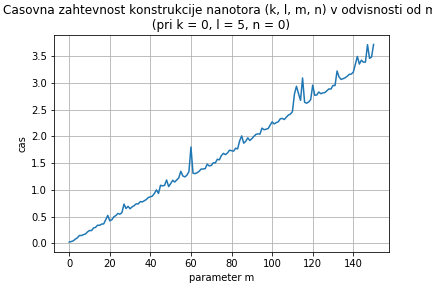
\includegraphics[width=10cm]{zahtevnost1}
\end{center}
\vspace{1cm}

Vidimo, da je časovna zahtevnost v tem primeru linearna, kar lahko pojanimo s tem, da se ob podaljševanju paralelograma v eno smer tudi mreža šestkotnikov poveča sorazmerno. Na naslednji sliki pa lahko vidimo, da v primeru podaljševanja paralelograma v dve različni smeri časovna zahtevnost funkcije raste kvadratično, saj se v tem primeru tudi mreža šestkotnikov povečuje v obe smeri.

\begin{center}
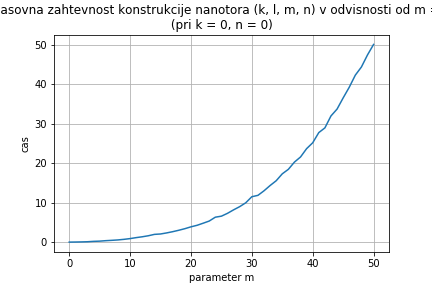
\includegraphics[width=10cm]{zahtevnost2}
\end{center}
\vspace{1cm}

\pagebreak


\section{Število točk do dane razdalje}

Število točk na razdaljah, krajših od danega $d$, sva dobila s sledečo funkcijo. Ob pisanju poročila sva ugotovila, da bi jo bilo mogoče optimizirati, če bi dodala množico že pregledanih vozlišč.

\begin{verbatim}
def vozlisca_na_razdalji_d(graf, start, dodane, d=0):
    # dodane je na zacetku prazna mnozica
    # start je vozlisce, kjer zacnemo
    if d == 0:
        dodane.add(start)
    elif d < 0:
        print("Negativna dolzina!")
    else:
        dodane.add(start)
        for povezava in graf[start]:
            vozlisca_na_razdalji_d(graf, povezava, dodane, d - 1)
    return dodane
\end{verbatim}


To funkcijo sva preizkusila na zelo različnih grafih z namenom, da bi našla formulo za izražanje števila točk z $d, k, l, m$ in $n$. Pri enostavnih grafih sva našla nekatere formule, ampak niso držale za vse razdalje. Na večjih grafih pa preprosto nisva uspela dobiti povezave, ki bi zajemala, kar se dogaja s številom točk pri spremembi parametrov. 

\begin{center}
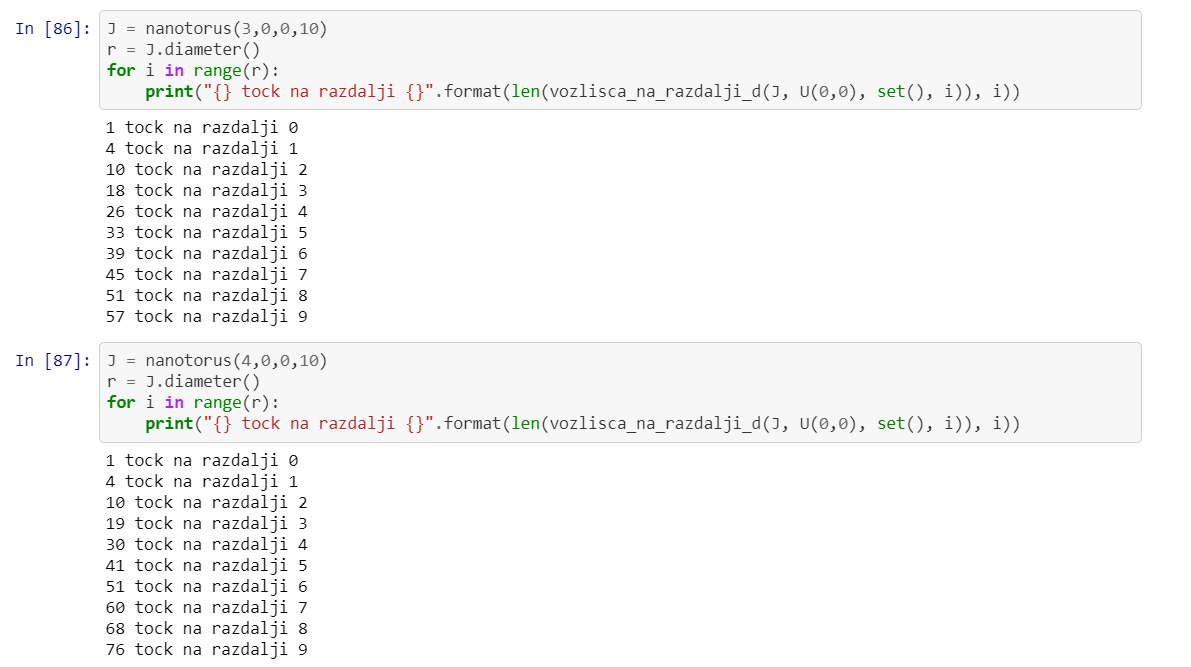
\includegraphics[width=10cm]{tocke}
\end{center}

\pagebreak

\section{Izomorfnost}

Nanotora bosta izomorfna, če na šestkotni mreži enačimo nekatere točke tako, da se bodo povezave med točkami ohranile. V najinem primeru sva želela dobiti graf oblike \texttt{(0, l', m', n')}, ki je izomorfen \texttt{(k, l, m, n)}. Tu sva navodila nekoliko priredila, saj sva v najinem programu zamenjala vektorja $A1$ in $A2$. V svojem bistvu ostaja naloga enaka, saj želiva zapisati nanotor \texttt{(k, l, m, n)} tako, da uničiva navpično komponento prvega vektorja. 
Ugotoviti sva morala, na kakšen način se začnejo poimenovanja točk na šestkotni mreži ponavljati zaradi enačenja nasprotnih stranic paralelograma. Želela sva dobiti vektor, ki v ''vodoravni'' smeri povezuje izhodišče mreže z naslednjo točko \texttt{U(0, 0)}. Ker se take točke nahajajo pri večkratnikih vektorjev \texttt{(k, l)} in \texttt{(m, n)}, ga lahko dobimo naslednjo enačbo: \texttt{a * (k, l) = b * (m, n) + (0, c)}. Velja: \texttt{a = m / d} in \texttt{b = k / d}, kjer je \texttt{d = gcd(m, k)}, pri čemer dovolimo, da se razlikuje v predznaku in dodamo zato absolutno vrednost. Dobimo, da je \texttt{c = abs(a * l - b * n)}.
Za izomorfna grafa mora veljati tudi, da lahko v točko \texttt{(m', n')} pridemo z neko kombinacijo vektorjev \texttt{(k, l)} in \texttt{(m, n)}, saj bomo tudi to točko enačili z \texttt{U(0,0)}. Iz tega sledi, da je \texttt{(m', n') = x * (k, l) + y * (m, n)}. Torej je \texttt{m' = gcd(m, k) = d} in \texttt{n' = x * l + y * n }.

Tako sva zapisala sledečo funkcijo, ki dani četverici \texttt{(k, l, m, n)} priredi \texttt{nanotorus(0, ll, mm, nn)}, izomorfen nanotorusu, ki ga dobimo s to četverico.

\begin{verbatim}
def izomorfni_graf(k, l, m, n):
    d, x, y = xgcd(k, m)
    d = abs(d)
    a = m / d
    b = k / d
    c = abs(a * l - b * n) # = (m * l - k * n) / d
    
    
    ll = c
    mm = d
    nn = x * l + y * n 
    
    return nanotorus(0, ll, mm, nn)
\end{verbatim}

\end{document}

